%\PassOptionsToClass{handout}{beamer}
\documentclass[english, aspectratio=169, sectionpage=true, onlytextwidth]{tumbeamer}
\usepackage[utf8]{inputenc}
\usepackage[T1]{fontenc}
\usepackage{babel}
\usepackage[bookmarks=true]{hyperref}
\usepackage{graphicx}
\usepackage[dvipsnames]{xcolor}
\usepackage{url}
\usepackage[useregional]{datetime2}
\usepackage{amsmath}
\usepackage{amssymb}
\usepackage{csquotes}[autostyle]

\subtitle[Bachelor's Thesis]{Bachelor's Thesis Colloquium}

\provideName{\theDepartmentName}
{School of Computation, Information and Technology}
{School of Computation, Information and Technology}

\provideName{\theChairName}
{Chair of Scientific Computing}
{Chair of Scientific Computing}

\institute{School of Computation, Information and Technology\\\theUniversityName}

%\footline{\insertauthor\enspace|\enspace\inserttitle\enspace|\enspace\insertdate}
\footline{\insertauthor\enspace|\enspace\insertsubtitle\enspace|\enspace\insertdate}

\graphicspath{ {./resources/} {./tumlatex/resources/} }


% macro to configure the style of the presentation
\TUMbeamersetup{
	content page = TUM default,  % style of normal content pages
%	content page = TUM more space,
}

\setbeamerfont{title}{size=\Large}

\AtBeginSection[]
{
	\begin{frame}
		\frametitle{Overview}
		\tableofcontents[sections=\value{section}]
	\end{frame}
}

\setbeamercolor{footnote}{fg=black}
\setbeamercolor{footnote mark}{fg=black}
\captionsetup{labelformat=empty}


% load additional packages
\usepackage{booktabs}
\usepackage{amsmath}
\usepackage{mathtools}
\usepackage{pmboxdraw}
\usepackage{float}
\usepackage{listings}
\usepackage{tikz}
\usepackage{pgf}
\usepackage{pgfplots}
\usepackage{float}
\usepackage{colortbl}
\usepackage{xcolor}
\usepackage{caption}

\usepackage{ulem}
\usepackage{enumerate}
\usepackage{pifont}
\usepackage{siunitx}
%\usepackage[scaled=0.85]{beramono} %better typewriter font

\definecolor{TUMBlue}{HTML}{0065BD}
\colorlet{chaptertumblue}{TUMBlue!60!black}

% Accent Colors
\definecolor{pred}{HTML}{F31124}
\definecolor{porange}{HTML}{FFA400}
\definecolor{pviolet}{HTML}{8E44AD}


\colorlet{tumblueaccdark}{chaptertumblue!80}
\colorlet{tumblueaccmedium}{chaptertumblue!50}
\colorlet{tumblueacclight}{chaptertumblue!30}
\colorlet{tumblueaccverylight}{chaptertumblue!10}
\colorlet{bluedarkoutline}{chaptertumblue}
\colorlet{bluedark}{chaptertumblue!80}
\colorlet{bluemedium}{chaptertumblue!50}
\colorlet{bluelight}{chaptertumblue!30}
\colorlet{blueverylight}{chaptertumblue!10}
\colorlet{reddark}{red!80}
\colorlet{orangedark}{porange!80}
\colorlet{violetdark}{pviolet!80}

\captionsetup{
	labelfont={bf,small},
	textfont={small}
} 
\captionsetup[sub]{labelfont=normal}


\pgfplotsset{compat=1.16}

% tikz
\usetikzlibrary{arrows,backgrounds,positioning,shapes,patterns,patterns.meta,matrix,arrows.meta,shapes.geometric,decorations.pathmorphing, matrix, fit, calc, overlay-beamer-styles, intersections}

%  unified tikz styling
\tikzset{
	barfilldark/.style={fill=bluedark, draw=bluedarkoutline},
	barfillmedium/.style={fill=bluemedium, draw=bluedarkoutline},
	barfillight/.style={fill=bluelight, draw=bluedarkoutline},
	barfillverylight/.style={fill=blueverylight, draw=bluedarkoutline},
	barfilldashed/.style={fill=none, draw=bluedarkoutline, customdash},
	accentRed/.style={draw=reddark},
	accentOrange/.style={draw=orangedark},
	accentViolet/.style={draw=violetdark},
	customdash/.style={dash pattern=on 2pt off 1pt},
	custombrace/.style={decorate,decoration={brace, amplitude=1ex, raise=0.5ex}},
}

\pgfplotsset{
	colormap={fast}{
		rgb255(0cm)=(14,14,119);
		rgb255(0.17159223942480895cm)=(61,117,206);
		rgb255(0.2984914818394138cm)=(90,189,243);
		rgb255(0.4321287371255907cm)=(175,237,234);
		rgb255(0.5cm)=(229,240,196);
		rgb255(0.5882260353170073cm)=(244,212,129);
		rgb255(0.7061412605695164cm)=(236,158,80);
		rgb255(0.8476395308725272cm)=(204,89,40);
		rgb255(1cm)=(150,19,30);
	}
}

\newcommand{\fastcolorbar}{%
	\centering
	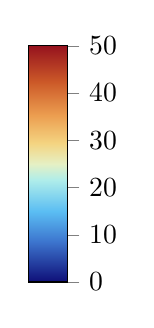
\begin{tikzpicture}
		\pgfplotscolorbardrawstandalone[
		colorbar,
		colormap name=fast,
		point meta min=0,
		point meta max=50,
		colorbar style={
			height=3cm,
			ytick={0,10,...,50},
			tick align=outside,
			tick pos=right,
		},
		]
	\end{tikzpicture}
	
	\begin{tikzpicture}
		\node[anchor=north, align=center] at (0,0) {\si{F^{*}}};
	\end{tikzpicture}
}

\newcommand{\fastcolorbarhor}{%
	\centering
	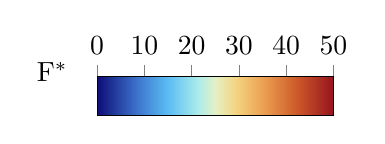
\begin{tikzpicture}
		\node[anchor=east, align=center] at (-0.25cm,-0.25cm) {\si{F^{*}}};
		\pgfplotscolorbardrawstandalone[
		colorbar horizontal,
		colormap name=fast,
		point meta min=0,
		point meta max=50,
		colorbar style={
			width=3cm,
			xtick={0,10,...,50},
			tick align=outside,
			tick pos=top,
			xticklabel pos=top,
		},
		]
	\end{tikzpicture}
}

\tikzset{
	linestyleA/.style={chaptertumblue, densely dotted, thick},
	linestyleB/.style={tumblueaccdark, densely dashed, thick},
	linestyleC/.style={tumblueaccmedium, solid, thick},
	linestyleD/.style={tumblueacclight, densely dashdotted, thick},
	linestyleE/.style={black, thin},
}

\pgfplotsset{
	triggerplot/.style={
		height=0.315\textwidth,
		width=0.45\textwidth,
		xlabel={Trigger Factor $\lambda$},
		xtick={1.25, 1.5, 1.75},
		legend style={font=\small},
		legend cell align=center,
		legend columns=3,
		legend style={at={(0.5,1.03)}, anchor=south, fill=none, draw=none, align=center},
		legend image post style={xscale=0.5},
		ylabel near ticks},
	logtriggerplot/.style={
		triggerplot,
		log basis y = 10,
		log ticks with fixed point}
}



% listings
\lstset{
	basicstyle=\ttfamily, 
	numbers=left,
	stepnumber=1,
	showstringspaces=false, 
	tabsize=4,
	breaklines=true, 
	breakatwhitespace=false,
	frame=single,
	captionpos=b, 
}

\graphicspath{ {../thesis/Figures} {../thesis/Figures/scenarios}}


%-------------------------------------------------------------------------------

\title{Adaptive Initiation of AutoPas Tuning\\Phases for Efficient Particle Simulations}
\date{\DTMdisplaydate{2025}{10}{01}{-1}}
\author{Niklas Ladurner}

\begin{document}

\maketitle

\begin{frame}[c]{Motivation}{}
	\begin{columns}
		\begin{column}{0.6\textwidth}
			\begin{itemize}
				\item AutoPas: automatic determination of simulation parameters
				\item Different scenarios have different optimal configurations
				\item Optimal configuration can change over time
				\item Currently: Tuning phases initiated at fixed intervals
				\item Improvement: Tuning phases initiated based on changes in simulation state
			\end{itemize}
		\end{column}
		\begin{column}{0.4\textwidth}
			% TODO: image
		\end{column}
	\end{columns}
\end{frame}

\begin{frame}[c, fragile]{Implementation}{}
	\only<1>{
		\begin{itemize}
			\item Based on runtime measurements of individual iterations
			\item Single parameter, only increases considered
			\item Four trigger strategies investigated:
			      \begin{enumerate}
				      \item \texttt{TimeBasedSimpleTrigger}
				      \item \texttt{TimeBasedAverageTrigger}
				      \item \texttt{TimeBasedSplitTrigger}
				      \item \texttt{TimeBasedRegressionTrigger}
			      \end{enumerate}
		\end{itemize}
	}
	\only<2,3>{
		\begin{figure}[htpb]
			\centering
			\def\barwidth{12pt}
			\pgfmathsetmacro{\lambdaval}{1.5}
			\begin{subfigure}{0.5\textwidth}
				\centering
				\resizebox{0.9\textwidth}{!}{
					\begin{tikzpicture}
						\begin{axis}[
								height=0.75\textwidth, width=\textwidth,
								xmin = -0.75,
								xmax = 8.75,
								ymin = 0,
								ymax = 2,
								xlabel={Iteration},
								ylabel={Iteration Runtime},
								ylabel near ticks,
								xtick={4,5},
								xticklabels={$i-1$,$i$},
								ytick=\empty,
								bar width=\barwidth,
								clip=false,
								legend pos=north east,
								xticklabel style={font={\scriptsize}},
								anchor=south
							]

							\addlegendimage{legend image code/.code={
										\draw[barfillverylight, anchor=center] (0cm, -0.15cm)  rectangle (0.3cm,0.15cm);
									}}
							\addlegendentry{\scriptsize$t_k$}
							\addlegendimage{legend image code/.code={
										\draw[barfilldashed, anchor=center] (0cm, -0.15cm)  rectangle (0.3cm,0.15cm);
									}}
							\addlegendentry{\scriptsize$\lambda t_{k-1}$}

							\addplot[ybar, barfillverylight] coordinates{
									(0,0.9)
									(1,1.17)
									(2,0.95)
									(3,1.1)
									(6,1.13)
									(7,1.33)
									(8,0.55)
								};
							\addplot[ybar, barfilldashed] coordinates{
									(1,0.9*\lambdaval)
									(2,1.17*\lambdaval)
									(3,0.95*\lambdaval)
									(4,1.1*\lambdaval)
								};
							\addplot[ybar, barfillmedium] coordinates {(4,0.9)};
							\addplot[ybar, barfilldark] coordinates {(5,1.7)};

							\draw[blueverylight, customdash, dash phase=0.9] ([xshift=-0.5*\barwidth]5, 0.9*\lambdaval) -- ([xshift=0.5*\barwidth]5, 0.9*\lambdaval);

							\draw [custombrace] ([xshift=-0.5*\barwidth]axis cs:6,2) -- (axis cs:8.75,2) node[midway, yshift=2.5ex]{New Tuning Phase};


						\end{axis}
						\node[yshift=-7ex] at (0, 0) {\texttt{TimeBasedSimpleTrigger}};
					\end{tikzpicture}
				}
			\end{subfigure}%
			\begin{subfigure}{0.5\textwidth}
				\centering
				\resizebox{0.9\textwidth}{!}{
					\begin{tikzpicture}[visible on=<3>]
						\begin{axis}[
								height=0.75\textwidth, width=\textwidth,
								xmin = -0.75,
								xmax = 8.75,
								ymin = 0,
								ymax = 2,
								xlabel={Iteration},
								ylabel={Iteration Runtime},
								ylabel near ticks,
								xtick={0,4,5},
								xticklabels={$i-n$,$i-1$,$i$,,},
								ytick=\empty,
								bar width=\barwidth,
								clip=false,
								legend pos=north west,
								xticklabel style={font={\scriptsize}},
								anchor=south
							]

							\addlegendimage{legend image code/.code={
										\draw[barfillverylight, anchor=center] (0cm, -0.15cm)  rectangle (0.3cm,0.15cm);
									}}
							\addlegendentry{\scriptsize$t_k$}

							\addlegendimage{legend image code/.code={
										\draw[fill=none, accentRed, thick, anchor=center] (0cm, 0cm) -- (0.3cm,0cm);
									}}
							\addlegendentry{\scriptsize$\phantom{\lambda}\text{avg}\left[t_{i-n}, t_{i-1}\right]$}

							\addlegendimage{legend image code/.code={
										\draw[barfilldashed, thick, anchor=center] (0cm, 0cm) -- (0.3cm,0cm);
									}}
							\addlegendentry{\scriptsize$\lambda \text{avg}\left[t_{i-n}, t_{i-1}\right]$}

							\addplot[ybar, barfillverylight] coordinates{
									(0,0.9)
									(1,1.17)
									(2,0.95)
									(3,1.1)
									(4,0.9)
									(6,1.13)
									(7,1.33)
									(8,0.55)
								};
							\addplot[ybar, barfilldark] coordinates {(5,1.7)};

							\draw[thick, accentRed] ([xshift=-0.5*\barwidth]axis cs: 0, 1.004) -- ([xshift=0.5*\barwidth]axis cs: 4, 1.004);

							% avg is 1,004
							\draw[draw=blueverylight, customdash, dash phase=0.9] ([xshift=-0.5*\barwidth]5, 1.004*\lambdaval) -- ([xshift=0.5*\barwidth]5, 1.004*\lambdaval);

							\draw [custombrace] ([xshift=-0.5*\barwidth]axis cs:6,2) -- (axis cs:8.75,2) node[midway, yshift=2.5ex]{New Tuning Phase};


						\end{axis}
						\node[yshift=-7ex] at (0, 0) {\texttt{TimeBasedAverageTrigger}};
					\end{tikzpicture}
				}
			\end{subfigure}
		\end{figure}
	}
	\only<4,5>{
		\begin{figure}[htpb]
			\centering
			\pgfmathsetmacro{\lambdaval}{1.25}
			\begin{subfigure}{0.5\textwidth}
				\centering
				\resizebox{0.9\textwidth}{!}{
					\begin{tikzpicture}
						\def\barwidth{6pt}
						\begin{axis}[
								height=0.75\textwidth, width=\textwidth,
								xmin = -0.75,
								xmax = 15.75,
								ymin = 0,
								ymax = 2,
								xlabel={Iteration},
								ylabel={Iteration Runtime},
								ylabel near ticks,
								xtick={0,5,11},
								xticklabels={$i-n$,$i-j$,$i$},
								ytick=\empty,
								bar width=\barwidth,
								clip=false,
								legend pos=north west,
								xticklabel style={font={\scriptsize}},
								anchor=south,
							]

							\addlegendimage{legend image code/.code={
										\draw[barfillverylight, anchor=center] (0cm, -0.15cm)  rectangle (0.3cm,0.15cm);
									}}
							\addlegendentry{\scriptsize$t_k$}
							\addlegendimage{legend image code/.code={
										\draw[accentRed, thick] (0cm, 0cm)  -- (0.3cm,0cm);
									}}
							\addlegendentry{\scriptsize$\phantom{\lambda}\text{avg}(A)$}
							\addlegendimage{legend image code/.code={
										\draw[accentViolet, thick] (0cm, 0cm)  -- (0.3cm,0cm);
									}}
							\addlegendentry{\scriptsize$\phantom{\lambda}\text{avg}(B)$}
							\addlegendimage{legend image code/.code={
										\draw[draw=chaptertumblue, thick, customdash] (0cm, 0cm)  -- (0.3cm,0cm);
									}}
							\addlegendentry{\scriptsize$\lambda\text{avg}(A)$}

							\pgfmathsetmacro{\k}{0.7}
							\pgfmathsetmacro{\xzero}{5}
							\pgfmathsetmacro{\yoff}{0.5}
							\pgfmathsetmacro{\yscale}{1.25}

							\addplot[ybar, barfillverylight, samples at={0,...,10,12,13,14,15}] {\yoff+\yscale/(1+exp(-\k*(x-\xzero)))};
							\addplot[ybar, barfilldark, samples at={11}] {\yoff +\yscale/(1+exp(-\k*(x-\xzero)))};

							\pgfmathsetmacro{\tmpsum}{0}
							\foreach \x in {0,...,5}{%
									\pgfmathparse{\tmpsum + \yoff + \yscale/(1 + exp(-\k*(\x-\xzero)))}%
									\global\let\tmpsum=\pgfmathresult%
								}
							\pgfmathsetmacro{\avgA}{\tmpsum/6}

							\pgfmathsetmacro{\tmpsum}{0}
							\foreach \x in {6,...,11}{%
									\pgfmathparse{\tmpsum + \yoff + \yscale/(1 + exp(-\k*(\x-\xzero)))}%
									\global\let\tmpsum=\pgfmathresult%
								}
							\pgfmathsetmacro{\avgB}{\tmpsum/6}

							\draw[thick, accentRed] ([xshift=-0.5*\barwidth]axis cs: 0, \avgA) -- ([xshift=0.5*\barwidth]axis cs: 5, \avgA);

							\draw[thick, accentViolet] ([xshift=-0.5*\barwidth]axis cs: 6, \avgB) -- ([xshift=0.5*\barwidth]axis cs: 11, \avgB);

							\draw[thick, customdash, bluedarkoutline] ([xshift=-0.5*\barwidth]axis cs: 6, \avgA*\lambdaval) -- ([xshift=0.5*\barwidth]axis cs: 11, \avgA*\lambdaval);

							\draw [custombrace] ([xshift=-0.5*\barwidth]axis cs:12,2) -- (axis cs:15.75,2) node[midway, yshift=2.5ex]{New Tuning Phase};


						\end{axis}
						\node[yshift=-7ex] at (0, 0) {\texttt{TimeBasedSplitTrigger}};
					\end{tikzpicture}
				}
			\end{subfigure}%
			\begin{subfigure}{0.5\textwidth}
				\centering
				\resizebox{0.9\textwidth}{!}{
					\begin{tikzpicture}[visible on=<5>]
						\def\barwidth{3pt}
						\begin{axis}[
								height=0.75\textwidth, width=\textwidth,
								xmin = -0.75,
								xmax = 23.75,
								ymin = 0,
								ymax = 2,
								xlabel={Iteration},
								ylabel={Iteration Runtime},
								ylabel near ticks,
								xtick={0,5,11},
								xticklabels={$i-n$,$i-j$,$i$},
								ytick=\empty,
								bar width=\barwidth,
								clip=false,
								legend pos=north west,
								xticklabel style={font={\scriptsize}},
								anchor=south,
							]

							\addlegendimage{legend image code/.code={
										\draw[barfillverylight, anchor=center] (0cm, -0.15cm)  rectangle (0.3cm,0.15cm);
									}}
							\addlegendentry{\scriptsize$t_k$}

							\addlegendimage{legend image code/.code={
										\draw[accentRed, thick] (0cm, 0cm)  -- (0.3cm,0cm);
									}}
							\addlegendentry{\scriptsize$\phantom{\lambda}t_\text{avg}$}
							\addlegendimage{legend image code/.code={
										\draw[accentViolet, thick] (0cm, 0cm)  -- (0.3cm,0cm);
									}}
							\addlegendentry{\scriptsize$\phantom{\lambda}t_\text{avg}^\text{proj}$}

							\addlegendimage{legend image code/.code={
										\draw[draw=bluedarkoutline, thick, customdash, anchor=center] (0cm, 0cm)  -- (0.3cm,0cm);
									}}
							\addlegendentry{\scriptsize$\lambda t_{\text{avg}}$}


							\pgfmathsetmacro{\k}{0.4}
							\pgfmathsetmacro{\xzero}{5}
							\pgfmathsetmacro{\yoff}{0.25}
							\pgfmathsetmacro{\yscale}{0.9}

							\draw[fill=none, draw=black, dotted, line join=round] ([xshift=-0.5*\barwidth]axis cs:12,1.08) -- ([xshift=0.5*\barwidth]axis cs: 23,1.98) -- ([xshift=0.5*\barwidth]axis cs: 23,1.08) -- cycle;


							\addplot[ybar, barfillverylight, samples at={0,...,10}] {\yoff+\yscale/(1+exp(-\k*(x-\xzero)))};
							\addplot[ybar,  barfilldark, samples at={11}] {\yoff +\yscale/(1+exp(-\k*(x-\xzero)))};
							\addplot[ybar, barfillverylight] coordinates {
									(12,0.39) (13,0.51) (14,0.31) (15,0.34) (16,0.40)
									(17,0.28) (18,0.64) (19,0.28) (20,0.29) (21,0.63)
									(22,0.67) (23,0.69)};

							\addplot[ybar, barfilldark, samples at={11}] {\yoff +\yscale/(1+exp(-\k*(x-\xzero)))};

							\pgfmathsetmacro{\tmpsum}{0}
							\foreach \x in {0,...,11}{%
									\pgfmathparse{\tmpsum + \yoff + \yscale/(1 + exp(-\k*(\x-\xzero)))}%
									\global\let\tmpsum=\pgfmathresult%
								}
							\pgfmathsetmacro{\avgA}{\tmpsum/12}

							\draw[thick, accentRed] ([xshift=-0.5*\barwidth]axis cs: 0, \avgA) -- ([xshift=0.5*\barwidth]axis cs: 11, \avgA);

							\draw[thick, accentViolet] ([xshift=-0.5*\barwidth]axis cs: 12, 1.53) -- ([xshift=0.5*\barwidth]axis cs: 23, 1.53);

							\draw[thick, customdash, bluedarkoutline] ([xshift=-0.5*\barwidth]axis cs: 11, \avgA*\lambdaval) -- ([xshift=0.5*\barwidth]axis cs: 23, \avgA*\lambdaval);


							\draw [custombrace] ([xshift=-0.5*\barwidth]axis cs:12,2) -- ([xshift=0.5*\barwidth]axis cs:23,2) node[midway, yshift=2.5ex]{New Tuning Phase};

							\draw [custombrace] ([yshift=-\pgflinewidth]axis cs:24,1.08) -- (axis cs:24,0) node[midway, align=left, anchor=west, xshift=1ex]{$t_i$};

							\draw [custombrace]  (axis cs:24,1.98) -- ([yshift=\pgflinewidth]axis cs:24,1.08) node[midway, align=left, anchor=west, xshift=1ex]{$\hat{\beta}_1't_i$};

						\end{axis}
						\node[yshift=-7ex] at (0, 0) {\texttt{TimeBasedRegressionTrigger}};
					\end{tikzpicture}
				}
			\end{subfigure}
		\end{figure}

	}
\end{frame}

% TODO: caption alignment across slides
\begin{frame}[c]{Evaluation}{}
	\only<1>{
		\begin{itemize}
			\item Three different evaluation scenarios:
			      \begin{enumerate}
				      \item Equilibrium
				      \item Exploding Liquid
				      \item Heating Sphere
			      \end{enumerate}
			\item Evaluation metrics:
			      \begin{enumerate}
				      \item Speedup (total runtime reduction)
				      \item Optimality (compared to static tuning intervals)
				      \item Number of tuning iterations
			      \end{enumerate}
		\end{itemize}
	}
	\only<2>{
		\begin{figure}[htpb]
			\centering
			\begin{subfigure}[c]{.25\textwidth}
				\includegraphics[width=\textwidth]{equilibrium/render/t0.png}
				\subcaption{Iteration \num{0}} % 0, 0
			\end{subfigure}%
			\begin{subfigure}[c]{.25\textwidth}
				\includegraphics[width=\textwidth]{equilibrium/render/t10000.png}
				\subcaption{Iteration \num{10000}} % 10000, 10
			\end{subfigure}%
			\begin{subfigure}[c]{.25\textwidth}
				\includegraphics[width=\textwidth]{equilibrium/render/t50000.png}
				\subcaption{Iteration \num{50000}} % 50000, 50
			\end{subfigure}%
			\begin{subfigure}[c]{.08\textwidth}
				\fastcolorbar
			\end{subfigure}
			\vspace{-0.3cm}
			\caption{Evolution of the simulation state in the equilibrium scenario.}
			\label{fig:evolution_equil}
		\end{figure}
	}
	\only<3>{
		\begin{figure}[htpb]
			\centering
			\begin{subfigure}[c]{.2\textwidth}
				\newsavebox{\colorbarbox}
				\savebox{\colorbarbox}{
					\fastcolorbarhor
				}
				\usebox{\colorbarbox}%
				\vspace*{-\ht\colorbarbox} %
				\includegraphics[width=\textwidth]{exploding-liquid/render/t0.png}
%				\vspace*{-\textwidth}
%				\vspace*{-0.25\textwidth}
				\vspace{-2cm}
				\subcaption{Iteration \num{0}} % 0 
			\end{subfigure}%
			\begin{subfigure}[c]{.2\textwidth}
				\includegraphics[width=\textwidth]{exploding-liquid/render/t3000.png}
				\vspace{-2cm}
				\subcaption{Iteration \num{3000}} % 3000, 5.5
			\end{subfigure}%
			\begin{subfigure}[c]{.2\textwidth}
				\centering
				\vspace{-1cm}
				\includegraphics[width=\textwidth]{exploding-liquid/render/t11000.png}
				\vspace{-1cm}
				\subcaption{Iteration \num{11000}} % 11000, 20
			\end{subfigure}%
			\begin{subfigure}[c]{.2\textwidth}
				\centering
				\vspace{-1cm}
				\includegraphics[width=\textwidth]{exploding-liquid/render/t31000.png}
				\vspace{-1cm}
				\subcaption{Iteration \num{31000}} % 31000, ?? 
			\end{subfigure}
			\vspace{-0.3cm}
			\caption{Evolution of the simulation state in the exploding-liquid scenario.}
		\end{figure}
	}
	\only<4>{
		\begin{figure}[htpb]
			\centering
			\newsavebox{\colorbarboxb}
			\savebox{\colorbarboxb}{
				\fastcolorbarhor
			}
			\vspace*{-1cm}
			\usebox{\colorbarboxb}%
			\vspace*{-\ht\colorbarboxb} %
			\vspace*{1cm}
			
			\begin{subfigure}{.25\textwidth}
				\includegraphics[draft=false,width=\textwidth]{heating-sphere/render/t0.png}
				\subcaption{Iteration \num{0}} % 0
			\end{subfigure}%
			\begin{subfigure}{.25\textwidth}
				\includegraphics[draft=false,width=\textwidth]{heating-sphere/render/t4000.png}
				\subcaption{Iteration \num{4000}} % 4000, 0.4
			\end{subfigure}%
			\begin{subfigure}{.25\textwidth}
				\includegraphics[draft=false,width=\textwidth]{heating-sphere/render/t23000.png}
				\subcaption{Iteration \num{23000}} % 23000, 2.3
			\end{subfigure}%
			\begin{subfigure}{.25\textwidth}
				\vspace*{0.1\textwidth}
				\centering
				\includegraphics[width=0.8\textwidth]{heating-sphere/render/t60000.png}
				\vspace*{0.1\textwidth}
				\subcaption{Iteration \num{60000}} % 60000, 6
			\end{subfigure}%
			\vspace{-0.3cm}
			\caption{Evolution of the simulation state in the heating-sphere scenario.}
		\end{figure}
	}
\end{frame}

% TODO
\begin{frame}[c]{Results}{}
	\only<1>{
		\begin{figure}[htpb]
		\centering
		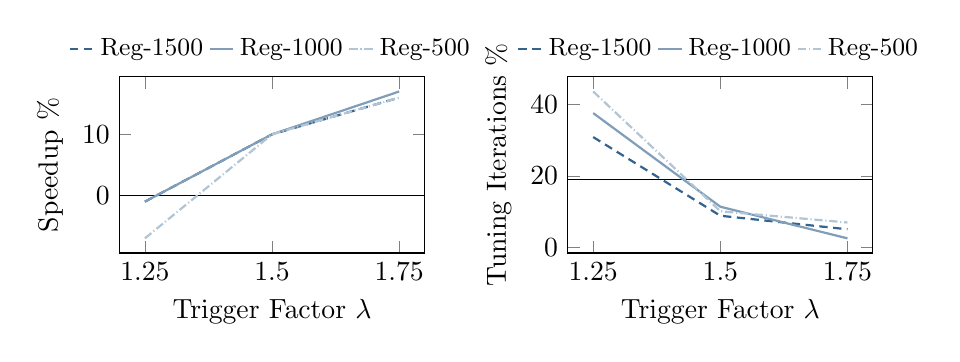
\begin{tikzpicture}
			\begin{axis}[
					triggerplot,
					name=baseplot3,
					trim axis left,
					legend columns=3,
					ylabel={Speedup \%},
				]
				% Baseline
				\draw[linestyleE] (axis cs:0,0) -- (axis cs: 2,0);

				% TimeBasedRegression 1500
				\addplot[linestyleB] coordinates{
						(1.25,-1)
						(1.5,10)
						(1.75,16)};

				% TimeBasedRegression 1000
				\addplot[linestyleC] coordinates{
						(1.25,-1)
						(1.5,10)
						(1.75,17)};

				% TimeBasedRegression 500		
				\addplot[linestyleD] coordinates{
						(1.25,-7)
						(1.5,10)
						(1.75,16)};

				\legend{Reg-1500,Reg-1000,Reg-500}
			\end{axis}

			\begin{axis}[
					logtriggerplot,
					at={(baseplot3.south east)},
					xshift=0.15\textwidth,
					trim axis left,
					legend columns=3,
					ylabel={Tuning Iterations \%},
					%				ymode=log,
					%				ymin=1,
					%				ymax=100,
				]
				% Baseline
				\draw[linestyleE] (axis cs:0,19.00) -- (axis cs: 2,19.00);

				% TimeBasedRegression 1500
				\addplot[linestyleB] coordinates{
						(1.25,30.92)
						(1.5,8.87)
						(1.75,5.07)};

				% TimeBasedRegression 1000
				\addplot[linestyleC] coordinates{
						(1.25,37.64)
						(1.5,11.4)
						(1.75,2.53)};

				% TimeBasedRegression 500		
				\addplot[linestyleD] coordinates{
						(1.25,43.7)
						(1.5,10.13)
						(1.75,6.97)};

				\legend{Reg-1500,Reg-1000,Reg-500}
			\end{axis}
		\end{tikzpicture}
		\caption{Regression trigger in the exploding-liquid scenario.}
	\end{figure}}
	\only<2>{
		\vspace{-0.75cm}
		\begin{figure}[htpb]
			\begin{subfigure}{0.45\textwidth}
				\centering
				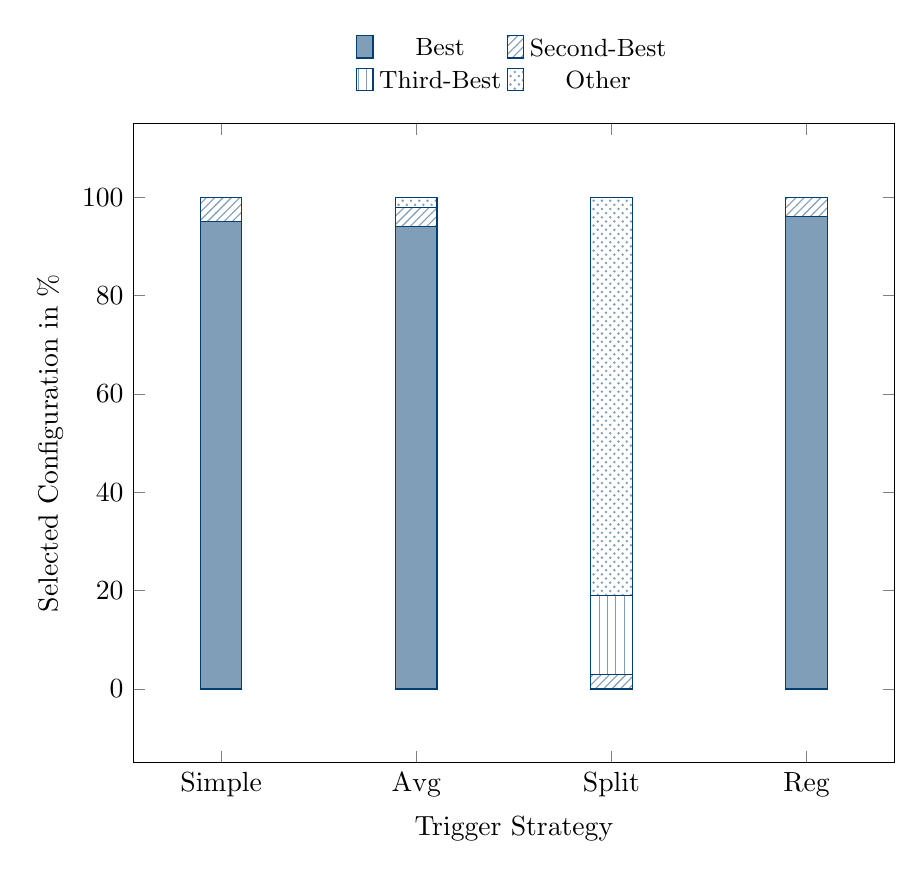
\begin{tikzpicture}
					\tikzset{
						barstyle1/.style={pattern color=tumblueaccmedium, draw=chaptertumblue,  pattern=crosshatch dots},
						barstyle2/.style={pattern color=tumblueaccmedium, draw=chaptertumblue, pattern=north east lines},
						barstyle3/.style={fill=tumblueaccmedium, draw=chaptertumblue},
						barstyle4/.style={pattern color=tumblueaccmedium, draw=chaptertumblue, pattern=vertical lines},
					}
					\def\barwidth{15pt}
					\begin{axis}[
							ybar stacked,
							height=0.8\textwidth,
							enlargelimits=0.15,
							ylabel={Selected Configuration in \unit{\percent}},
							xlabel={Trigger Strategy},
							symbolic x coords={Simple,Avg,Split,Reg},
							xtick=data,
							bar width=\barwidth,
							legend style={font=\small, nodes={yshift=0.25ex}},
							legend cell align=center,
							legend columns=2,
							legend style={at={(0.5,1.03)}, anchor=south, fill=none, draw=none, align=center},
						]
						% Top 1
						\addplot+[ybar, barstyle3] plot coordinates {(Simple,95) (Avg,94)
								(Split,0) (Reg,96)};

						% Top 2
						\addplot+[ybar, barstyle2] plot coordinates {(Simple,5) (Avg,4)
								(Split,3) (Reg,4)};

						% Top 3
						\addplot+[ybar, barstyle4] plot coordinates {(Simple,0) (Avg,0)
								(Split,16) (Reg,0)};

						% Other
						\addplot+[ybar, barstyle1] plot coordinates {(Simple,0) (Avg,2)
								(Split,81) (Reg,0)};

						\legend{Best,Second-Best,Third-Best,Other}
					\end{axis}
				\end{tikzpicture}
			\end{subfigure}%
			\begin{subfigure}{0.45\textwidth}
				\vskip 0pt
				\centering
				\includegraphics[width=\textwidth]{plots/exploding-liquid_configs_static.pdf}
				\vspace*{-1.075cm}
			\end{subfigure}
			\vspace{0.1cm}
			\caption{Configuration choice in the exploding-liquid scenario.}
			\label{fig:expl_optimality}
		\end{figure}
	}
	\only<3>{
		\vspace{-0.25cm}
		\begin{figure}[htpb]
			\begin{subfigure}[]{0.45\textwidth}
				\vskip 0pt
				\centering
				% equilibrium_dynamic_TimeBasedAverage_1.25_1000
				\includegraphics[width=\textwidth]{plots/exploding-liquid_configs_good.pdf}
			\end{subfigure}%
			\begin{subfigure}[]{0.45\textwidth}
				\vskip 0pt
				\centering
				% equilibrium_dynamic_TimeBasedSimple_1.25_10
				\includegraphics[width=\textwidth]{plots/exploding-liquid_configs_bad.pdf}
			\end{subfigure}
			\vspace{-0.5cm}
			\caption{Examples of trigger behavior in the exploding-liquid scenario.}
			\label{fig:expl_trigger_behavior}
		\end{figure}}
\end{frame}

\begin{frame}[c]{Conclusion}{}
	\begin{itemize}
		\item Four novel dynamic trigger strategies
		\item Best speedup: \qty{47}{\percent} (equilibrium)
		\item Better than static intervals with \texttt{full-search} in suitable scenarios
		\item Suboptimal if no indicated change in iteration runtime (e.g. heating-sphere)
		\item Good configuration fit
		\item Cheaper tuning phases $\rightarrow$ dynamic tuning less relevant
		\item Still useful for MPI-parallel applications
	\end{itemize}
\end{frame}


\begin{frame}[c]{}{}
	\begin{center}
		\LARGE Questions
	\end{center}
\end{frame}

\maketitle

\end{document}
